\documentclass[
		11pt,
		a4paper,
		toc=listof, %% Abbildungs- und Tabellenverzeichnis mit ins Inhaltsverzeichnis
		bibliography=totoc %% Quellenverzeichnis mit ins Inhaltsverzeichnis
		]{scrreprt}	 %% KOMA Script

% HTWG
\usepackage{graphicx}
\usepackage{a4}
\usepackage{german}
\selectlanguage{english}

% Eigene
\usepackage[utf8]{inputenc} %% Umlaute
\usepackage[printonlyused]{acronym} %% Abkuerzungsverzeichnis (nur verwendete)
\usepackage[colorinlistoftodos,prependcaption,textsize=tiny]{todonotes} %% TODOs moeglich mit \todo{}
\usepackage{booktabs} %% Tabellen
\usepackage{amsmath} %% Formeln
\usepackage{listings} %% Codebeispiele
\usepackage{subfigure} %% Mehrere Bilder nebeneinander
\usepackage[hyphens,spaces,obeyspaces]{url}

\usepackage{verbatim} %% multiline comments \begin{comment} hello world \end{comment}
\usepackage{csquotes}
\usepackage{enumitem}
\usepackage{multicol}


\usepackage[absolute]{textpos}

\usepackage{rotating}
\usepackage{booktabs}

\usepackage{tabularx}

\usepackage{float}

% Eigenes Design
%TODO loeschen wenn default HTWG Design (was es nicht wirklich gibt) gewuenscht ist
\usepackage[bottom=3cm]{geometry}
\usepackage{setspace}
\onehalfspacing

\usepackage{xargs}                      % Use more than one optional parameter in a new commands

% KOMA script anpassungen
%TODO entfernen wenn kein KOMA Script gewuenscht
\usepackage{scrhack}


%%%%%%%% Codebeispiele
\usepackage{color}
\usepackage{xcolor}  % Coloured text etc.
\usepackage{listings}
\usepackage{caption}


\newcommandx{\unsure}[2][1=]{\todo[linecolor=red,backgroundcolor=red!25,bordercolor=red,#1]{#2}}
\newcommandx{\change}[2][1=]{\todo[linecolor=blue,backgroundcolor=blue!25,bordercolor=blue,#1]{#2}}
\newcommandx{\info}[2][1=]{\todo[linecolor=OliveGreen,backgroundcolor=OliveGreen!25,bordercolor=OliveGreen,#1]{#2}}
\newcommandx{\improvement}[2][1=]{\todo[linecolor=yellow,backgroundcolor=yellow!25,bordercolor=yellow,#1]{#2}}
\newcommandx{\thiswillnotshow}[2][1=]{\todo[disable,#1]{#2}}

\usepackage[para]{bigfoot}\DeclareNewFootnote[para]{default} %% Footnodes next to each other

\setcounter{tocdepth}{2}  %% Ueberschriften bis subsection ins Inhaltsverzeichnis
\setcounter{secnumdepth}{3}  %% Nummerierung bis subsection


%%% Codebeispiele - Style
\DeclareCaptionFont{white}{\color{white}}
\DeclareCaptionFormat{listing}{\colorbox{gray}{\parbox{\textwidth}{#1#2#3}}}
\captionsetup[lstlisting]{format=listing,labelfont=white,textfont=white}

% Entfernt Kapitel Ueberschrift
% Bsp.
% 	ALT:
%       Kapitel 1
%       Einführung
%
% 	NEU:
% 		1 Einführung
%
\renewcommand*\chapterheadstartvskip{\vspace{-\topskip}}

\begin{comment}
    % removes indentation of paragraphs
    \setlength{\parindent}{0pt}
\end{comment}

\begin{comment}
    % creates footnotes for the first use of an acronym
    \makeatletter
    \renewcommand{\ac}{\protect\@ac}%
    \renewcommand{\@ac}[1]{%
        \expandafter\ifx\csname ac@#1\endcsname\AC@used
            \acs{#1}%
        \else \acs{#1}\footnote{\acl{#1}}%
            \global\expandafter\let\csname ac@#1\endcsname\AC@used%
            \AC@addtoAC@clearlist{#1}%
            \AC@logged{#1}
        \fi
    }
    \makeatother
\end{comment}

\newcommand{\thema}{$[$Thema der Bachelorarbeit$]$}
\newcommand{\schlagworte}{$[$Platz, f\"ur, spezifische, Schlagworte, zur, Ausarbeitung $]$}
\newcommand{\zusammenfassung}{$[$Text der Zusammenfassung etwa 150 Worte. Es soll der
	L"osungsweg beschrieben sein.$]$}
\newcommand{\ausgabedatum}{$[$Datum$]$}
\newcommand{\abgabedatum}{$[$Datum$]$}
\newcommand{\autor}{$[$Vor- und Zuname des/der Bachelorkandidaten/in$]$}
\newcommand{\autorStrasse}{$[$Stra"se$]$}
\newcommand{\autorPLZ}{$[$PLZ$]$}
\newcommand{\autorOrt}{$[$Ort$]$}
\newcommand{\autorGeburtsort}{$[$Geburtsort$]$}
\newcommand{\autorGeburtsdatum}{$[$Datum$]$}
\newcommand{\prueferA}{$[$Titel, Vor- und Zuname des 1. Pr"ufers$]$}
\newcommand{\prueferB}{$[$Titel, Vor- und Zuname des 2. Pr"ufers$]$}
\newcommand{\firma}{$[$HTWG oder Firmenname$]$}
\newcommand{\studiengang}{$[$Software-Engineering/Technische Informatik/Wirtschaftsinformatik$]$}

\definecolor{lightgray}{rgb}{.9,.9,.9}
\definecolor{darkgray}{rgb}{.2,.2,.2}
\definecolor{purple}{rgb}{0.65, 0.12, 0.82}

\lstdefinelanguage{JavaScript}{
	keywords={typeof, new, true, false, catch, function, return, null, catch, switch, var, if, in, while, do, else, case, break},
	keywordstyle=\color{blue}\bfseries,
	ndkeywords={class, export, boolean, throw, implements, import, this},
	ndkeywordstyle=\color{darkgray}\bfseries,
	identifierstyle=\color{black},
	sensitive=false,
	tabsize=2,
	extendedchars=true,
	inputencoding=utf8,
	comment=[l]{//},
	morecomment=[s]{/*}{*/},
	commentstyle=\color{purple}\ttfamily,
	stringstyle=\color{red}\ttfamily,
	morestring=[b]',
	morestring=[b]"
}


\begin{document}
%% Nummerierung aus
\pagenumbering{gobble}

% HTWG Tempaltes fuer Titelseite etc.
\begin{titlepage}

\vspace*{-3.5cm}

\begin{flushleft}
\hspace*{-1cm} 
\includegraphics{htwg/htwg_in_pos_2}
\end{flushleft}


\begin{textblock*}{288mm}(123mm,9mm)

\includegraphics[]{htwg/htwg_in_pos_1}
\end{textblock*}


\vspace{2.0cm}

\begin{center}
	\huge{
		\textbf{\thema} \\[5cm]
	}
	\Large{
		\textbf{\autor}} \\[5.5cm]
	\large{
		\textbf{Konstanz, \abgabedatum} \\[2.3cm]
	}

	\Huge{
		\textbf{Bachelorarbeit}
	}
\end{center}

\end{titlepage}

\thispagestyle{empty}
{
\setlength{\parskip}{0.5cm}
        \begin{center}
        \textbf{\huge BACHELORARBEIT}

        \textbf{zur Erlangung des akademischen Grades}

        \textbf{\Large Bachelor of Science (B. Sc.)}

        \textbf{an der}

        \textsf{\huge Hochschule Konstanz}\\
        {\small Technik, Wirtschaft und Gestaltung}

        \textsf{\Large Fakult"at Informatik} \\
        Studiengang \studiengang
        \end{center}
}
\begin{center}

\vspace*{1.4cm}

\begin{tabular}{p{3cm}p{10cm}}
Thema: & \textbf{\large \thema} \\[15ex]
Bachelorkandidat: & \autor, \autorStrasse, \autorPLZ{}  \autorOrt{} \\[15ex]
1. Pr"ufer: & \prueferA \\
2. Pr"ufer: & \prueferB \\[25ex]
Ausgabedatum: & \ausgabedatum \\
Abgabedatum: & \abgabedatum \\
\end{tabular}
\end{center}

\begin{center}
{\Large \textbf{Zusammenfassung (Abstract)}}
\end{center}

\bigskip

\begin{center}
	\begin{tabular}{p{4cm}p{9cm}}
		Thema: & \thema \\
		 & \\
		Bachelorkandidat: & \autor \\
		 & \\
		Firma: & \firma \\
		 & \\
		Betreuer: & \prueferA  \\[.5ex]
		 &  \prueferB \\
		 & \\
		Abgabedatum: & \abgabedatum \\
		 & \\
		Schlagworte: & \schlagworte \\
		 & \\
	\end{tabular}
\end{center}

\bigskip

\noindent
\zusammenfassung


\pagenumbering{Roman}
\chapter*{Ehrenw"ortliche Erkl"arung}

Hiermit erkl"are ich
\textit{\autor, geboren am \autorGeburtsdatum{} in \autorGeburtsort{}}, dass ich\\

\begin{tabular}{lp{12cm}}
(1) & meine Bachelorarbeit mit dem Titel \\[1em]
& \textbf{\thema} \\[1em]
& bei der \firma\ unter Anleitung von \prueferA\ selbst"andig und ohne fremde Hilfe angefertigt und keine anderen als die angef"uhrten Hilfen benutzt habe;\\[1em]
(2) & die "Ubernahme w"ortlicher Zitate, von Tabellen, Zeichnungen, Bildern und
Programmen aus der Literatur oder anderen Quellen (Internet) sowie die Verwendung
der Gedanken anderer Autoren an den entsprechenden Stellen innerhalb der Arbeit
gekennzeichnet habe.\\
\end{tabular}

\vspace*{1cm}

\noindent
Ich bin mir bewusst, dass eine falsche Erkl"arung rechtliche Folgen haben wird.\\

\vspace*{3cm}

\noindent
Konstanz, \abgabedatum \hfill \begin{tabular}{c} \\ \\ \rule{5cm}{1pt} \\ (Unterschrift)\end{tabular}

\begin{comment}
    % optional non fixed date, if someone submits his/her thesis before deadline
    \begin{tabular}{ c@{\hskip 1.6in}c }
    	\rule{5cm}{1pt} & \rule{5cm}{1pt} \\
    	(Ort, Datum) & (Unterschrift)
    \end{tabular}
\end{comment}


\tableofcontents

%!TEX root = thesis.tex

\chapter*{Abkürzungsverzeichnis}
\addcontentsline{toc}{chapter}{Abkürzungsverzeichnis}

\begin{acronym}
 \acro{HTTP} {Hypertext Transfer Protocol}
\end{acronym}

\newcounter{prepend}
\setcounter{prepend}{\value{page}} % save page count for appendix

%% Starte Paginierung
\cleardoublepage
\pagenumbering{arabic}

%!TEX root = ../thesis.tex

\chapter{Einführung}

Lorem ipsum dolor sit amet, consetetur sadipscing elitr, sed diam nonumy eirmod tempor invidunt ut labore et dolore magna aliquyam erat, sed diam voluptua. At vero eos et accusam et justo duo dolores et ea rebum. Stet clita kasd gubergren, no sea takimata sanctus est Lorem ipsum dolor sit amet. Lorem ipsum dolor sit amet, consetetur sadipscing elitr, sed diam nonumy eirmod tempor invidunt ut labore et dolore magna aliquyam erat, sed diam voluptua. At vero eos et accusam et justo duo dolores et ea rebum. Stet clita kasd gubergren, no sea takimata sanctus est Lorem ipsum dolor sit amet.

\section{tbd} 

Lorem ipsum dolor sit amet, consetetur sadipscing elitr, sed diam nonumy eirmod tempor invidunt ut labore et dolore magna aliquyam erat, sed diam voluptua. At vero eos et accusam et justo duo dolores et ea rebum. Stet clita kasd gubergren, no sea takimata sanctus est Lorem ipsum dolor sit amet. Lorem ipsum dolor sit amet, consetetur sadipscing elitr, sed diam nonumy eirmod tempor invidunt ut labore et dolore magna aliquyam erat, sed diam voluptua. At vero eos et accusam et justo duo dolores et ea rebum. Stet clita kasd gubergren, no sea takimata sanctus est Lorem ipsum dolor sit amet.

\section{tbd} 
Lorem ipsum dolor sit amet, consetetur sadipscing elitr, sed diam nonumy eirmod tempor invidunt ut labore et dolore magna aliquyam erat, sed diam voluptua. At vero eos et accusam et justo duo dolores et ea rebum. Stet clita kasd gubergren, no sea takimata sanctus est Lorem ipsum dolor sit amet. Lorem ipsum dolor sit amet, consetetur sadipscing elitr, sed diam nonumy eirmod tempor invidunt ut labore et dolore magna aliquyam erat, sed diam voluptua. At vero eos et accusam et justo duo dolores et ea rebum. Stet clita kasd gubergren, no sea takimata sanctus est Lorem ipsum dolor sit amet.


%!TEX root = ../thesis.tex

\chapter{Grundlagen}

\ac{LOL} Lorem ipsum dolor sit amet, consetetur sadipscing elitr, sed diam nonumy eirmod tempor invidunt ut labore et dolore magna aliquyam erat, sed diam voluptua. At vero eos et accusam et justo duo dolores et ea rebum. Stet clita kasd gubergren, no sea takimata sanctus est Lorem \ac{HTTP} ipsum dolor sit amet. Lorem ipsum dolor sit amet, consetetur sadipscing elitr, sed diam nonumy eirmod tempor invidunt ut labore et dolore magna aliquyam erat, sed diam voluptua. At vero eos et accusam et justo duo dolores et ea rebum. Stet clita kasd gubergren, no sea takimata sanctus est Lorem ipsum dolor sit amet.

\section{tbd} 

Lorem ipsum dolor sit amet, consetetur sadipscing elitr, sed diam nonumy eirmod tempor invidunt ut labore et dolore magna aliquyam erat, sed diam voluptua. At vero eos et accusam et justo duo dolores et ea rebum. Stet clita kasd gubergren, no sea takimata sanctus est Lorem ipsum dolor sit amet. Lorem ipsum dolor sit amet, consetetur sadipscing elitr, sed diam nonumy eirmod tempor invidunt ut labore et dolore magna aliquyam erat, sed diam voluptua. At vero eos et accusam et justo duo dolores et ea rebum. Stet clita kasd gubergren, no sea takimata sanctus est Lorem ipsum dolor sit amet.

\subsection{tbd} 
Lorem ipsum dolor sit amet, consetetur sadipscing elitr, sed diam nonumy eirmod tempor invidunt ut labore et dolore magna aliquyam erat, sed diam voluptua. At vero eos et accusam et justo duo dolores et ea rebum. Stet clita kasd gubergren, no sea takimata sanctus est Lorem ipsum dolor sit amet. Lorem ipsum dolor sit amet, consetetur sadipscing elitr, sed diam nonumy eirmod tempor invidunt ut labore et dolore magna aliquyam erat, sed diam voluptua. At vero eos et accusam et justo duo dolores et ea rebum. Stet clita kasd gubergren, no sea takimata sanctus est Lorem ipsum dolor sit amet.

\subsubsection{tbd} 
Lorem ipsum dolor sit amet, consetetur sadipscing elitr, sed diam nonumy eirmod tempor invidunt ut labore et dolore magna aliquyam erat, sed diam voluptua. At vero eos et accusam et justo duo dolores et ea rebum. Stet clita kasd gubergren, no sea takimata sanctus est Lorem ipsum dolor sit amet. Lorem ipsum dolor sit amet, consetetur sadipscing elitr, sed diam nonumy eirmod tempor invidunt ut labore et dolore magna aliquyam erat, sed diam voluptua. At vero eos et accusam et justo duo dolores et ea rebum. Stet clita kasd gubergren, no sea takimata sanctus est Lorem ipsum dolor sit amet.


%!TEX root = ../thesis.tex

\chapter{Codebeispiel}

Lorem ipsum dolor sit amet, consetetur sadipscing elitr, sed diam nonumy eirmod tempor invidunt ut labore et dolore magna aliquyam erat, sed diam voluptua. At vero eos et accusam et justo duo dolores et ea rebum. Stet clita kasd gubergren, no sea takimata sanctus est Lorem ipsum dolor sit amet.

\section{tbd} 


Referenz aufs Codebeispiel \ref{code}.

\lstinputlisting[language=Java,label=code,caption=Codebeispiel Java]{kapitel3/minimalSpringBoot.java}

\section{Highlighting}

\lstinputlisting[language=JavaScript,label=highlightjs,caption=JavaScript Highlighting]{kapitel3/example.js}
%!TEX root = ../thesis.tex

\chapter{Bilder}

Lorem ipsum dolor sit amet, consetetur sadipscing elitr, sed diam nonumy eirmod tempor invidunt 
\section{Ein Bild ganz breit} 
Verweis auf das Beispielbild \ref{fig:zuul}

\begin{figure}[htbp]
 \centering
 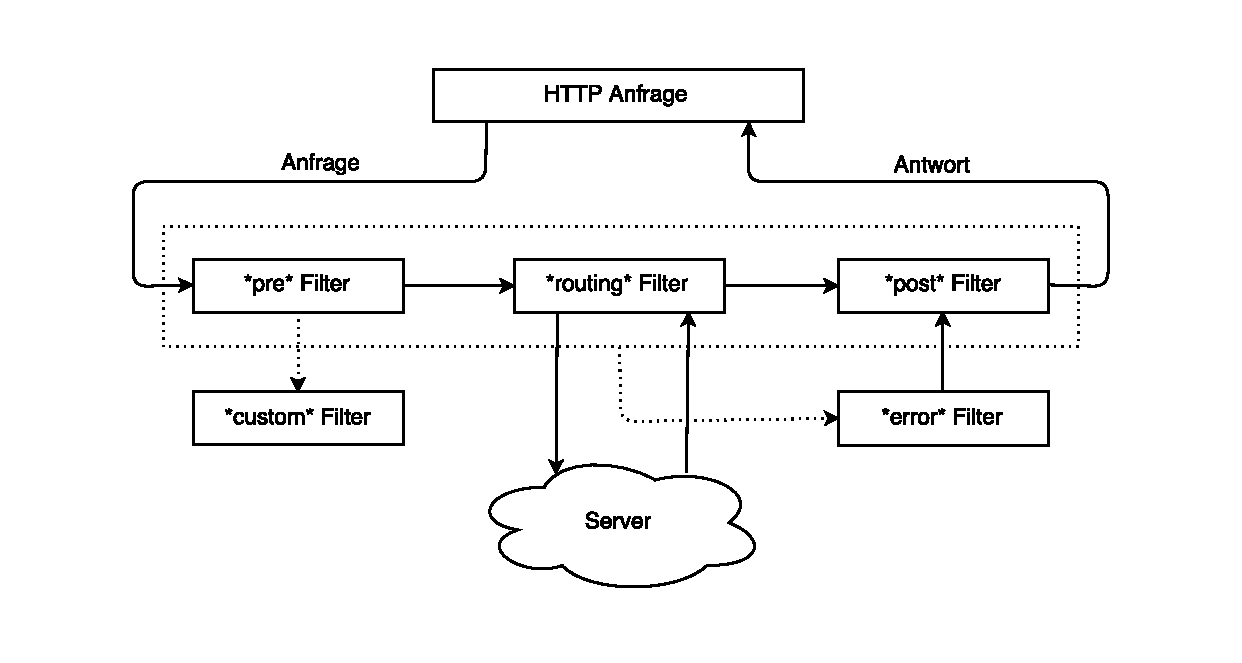
\includegraphics[width=\linewidth]{kapitel3/bilder/beispielbild}
 \caption{Beispielbild}
 \label{fig:zuul}
\end{figure}


\section{Zwei Bilder nebeneinander} 


\begin{figure}
\subfigure[Antwortzeiten]{\label{fig:antwortzeit}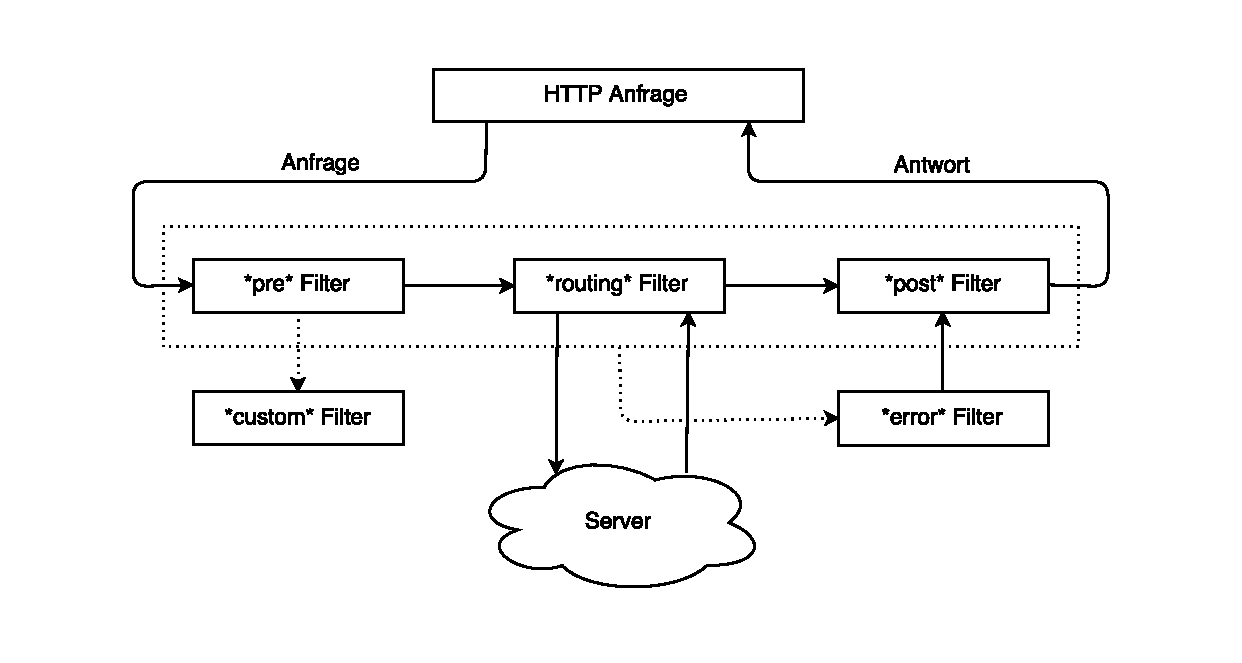
\includegraphics[width=0.50\textwidth]{kapitel3/bilder/beispielbild}}\hfill
\subfigure[prozentualer Anteil an fehlerhaften Anfragen]{\label{fig:fehler}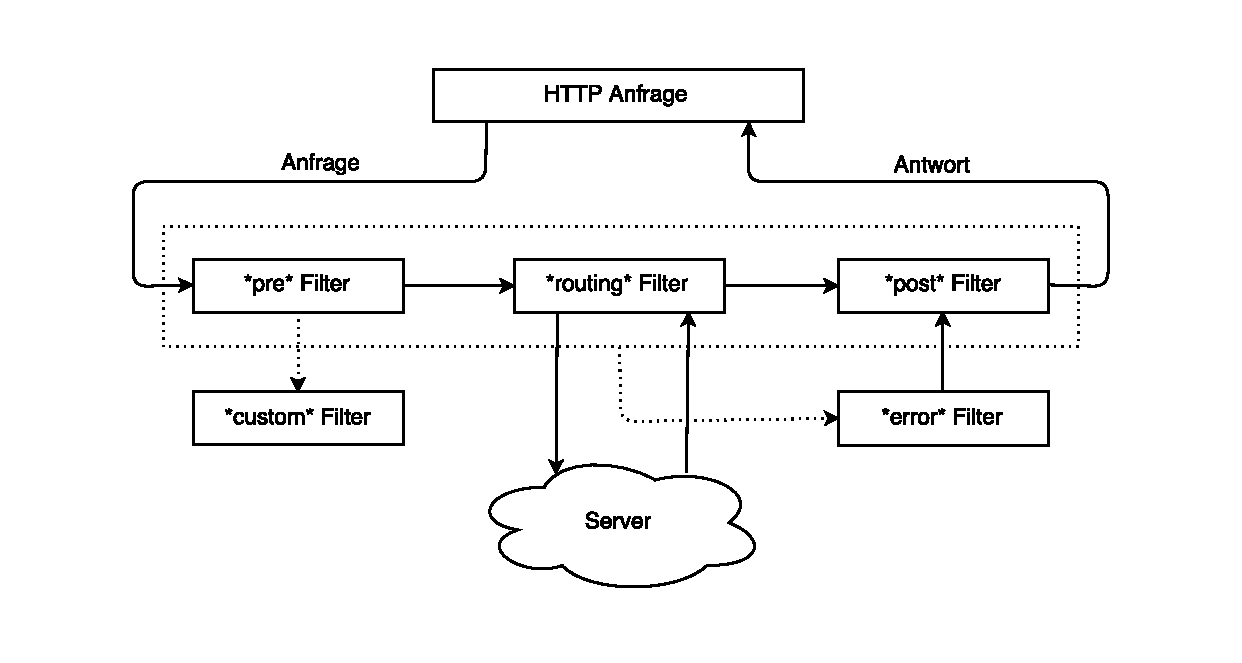
\includegraphics[width=0.50\textwidth]{kapitel3/bilder/beispielbild}}
\caption{Lasttest Szenarien}
\end{figure}

\newpage
\section{Bild mit Quellenangabe in der Fusszeile}

\begin{figure}[h]
	\centering
	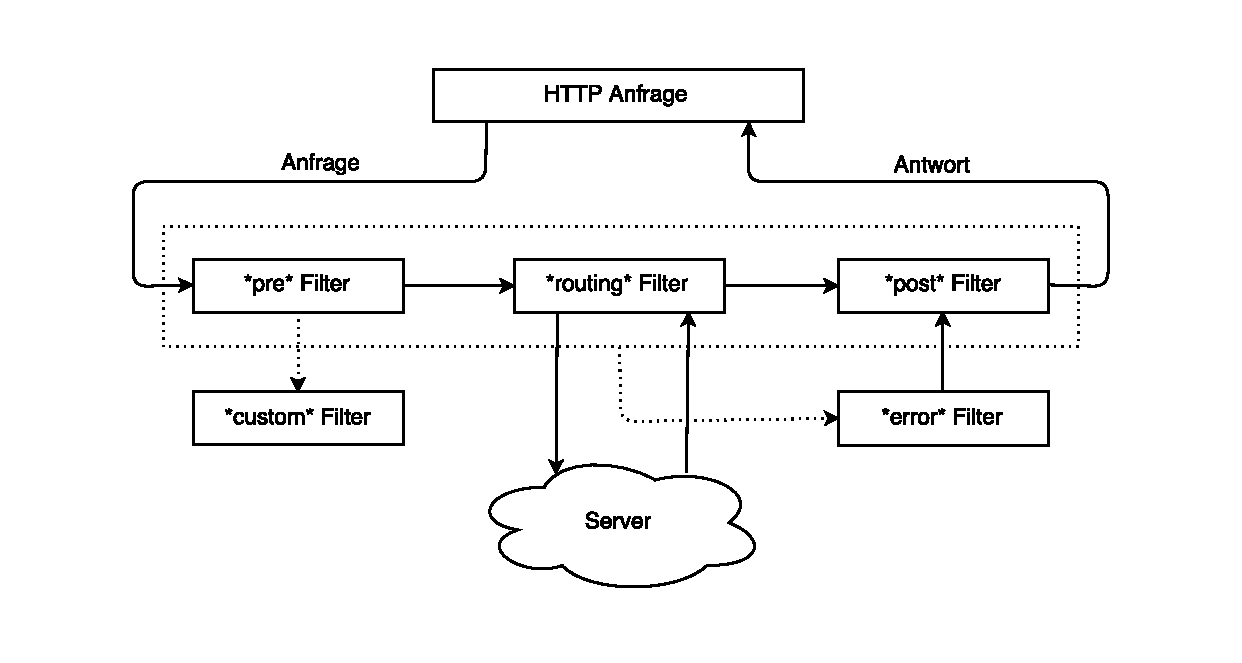
\includegraphics[width=\linewidth]{kapitel3/bilder/beispielbild}
	\caption[Beispielbild mit Qellenangabe in der Fusszeile]{Beispielbild mit Qellenangabe in der Fusszeile\protect\footnotemark}
\end{figure}
\footnotetext{Quelle: https://foo.bar/beispielbild.jpg}
%!TEX root = ../thesis.tex

\chapter{Tabelle}

Generierbar mit \url{http://www.tablesgenerator.com/}

\section{tbd} 

\begin{table}[h]
\centering
\caption{Ergebnisse des Integrationstests in Sekunden}
\label{tab:integration}
\begin{tabular}{@{}ccccc@{}}
\toprule
Testszenario    & Start  & Registrierung & 1. Nachricht & \textbf{Gesamt} \\ \midrule
Integration\_01 & 14,598 & 10,079        & 45,449       & 70,026        \\
Integration\_02 & 14,485 & 10,108        & 54,382       & 79,088        \\
Integration\_03 & 14,498 & 10,055        & 55,125       & 79,678        \\
Integration\_04 & 14.598 & 5,361         & 36,655       & 56,614          \\ \bottomrule
\end{tabular}
\end{table}
%!TEX root = ../thesis.tex

\chapter{Quellen verwenden / verwalten}

Am besten http://www.citeulike.org/ verwenden und Exportieren als bibtex Datei.


\section{Verwenden}

Beispiel - Typ: apalike


Ergebnis: \cite{haase}

\pagenumbering{Roman}
\setcounter{page}{\value{prepend} + 1} % continue roman page count for appendix

\listoffigures
\lstlistoflistings
\listoftables

\nocite{*} % adds all references without citations to bibliography
\bibliographystyle{apalike}
\bibliography{citeulike}

%!TEX root = ../thesis.tex

\chapter*{Anhang}
\addcontentsline{toc}{chapter}{Anhang}

Auf der beiliegenden CD befinden sich die folgenden Daten:
\begin{itemize}
	\item Dieses Dokument im PDF-Format
	\item ...
\end{itemize}

\end{document}
